\chapter{Implementation\label{cha:chapter5}}

This chapter describes the implementation of component X. Three systems were chosen as reference implementations: a desktop version for Windows and Linux PCs, a Windows Mobile version for Pocket PCs and a mobile version based on Android. 

\section{Completing the Scale Tezos Blockchain with Zk-Rollups project}
This section explains the implementation of the remaining features of the Scale Tezos Blockchain with Zk-Rollups project. Since some other already-implemented features have been modified, this section also explains the changes made to those features.

\subsection{Storage}

The storage has been modified to support a growing number of users. The accounts that are holding the proprieties of \textit{Public Key}, \textit{Balance} and \textit{Nonce} are now saved as a Big Map. It differs from the previous implementation where accounts were saved in a Map. This is a key difference because the Big Map is lazily deserialized\footnote{\url{https://tezos.gitlab.io/michelson-reference/\#type-big_map}}, not having to use gas during a contract call to deserialize all the accounts Map.

\subsection{Rollup execution}

The rollup execution has changed to include the calculation of the new nonces of the users. This is done while checking the transaction nonces. A precondition that must be respected is that Zokrates receives the transaction ordered by nonce for a user. It can receive transactions from different users but the transactions of a single user must be ordered by nonce. The algorithm that checks the transaction nonces and calculates the new nonces is the following:
\begin{itemize}
	\item Create an array copying the total nonce array;
	\item Iterate over the transactions:
	\item \begin{itemize}
		\item Check if the transaction nonce is equal to the nonce of the user plus 1;
		\item If it is, increment the nonce of the user in the array and continue;
		\item If it is not, fail execution.
    \end{itemize}
\end{itemize}

This allows to receive multiple transactions from the same user.

No relevant overhead is added to the complexity of the rollup execution because the nonce check is done in the same loop of the balance calculation, it is still O(n).

\subsection{Balance and Nonce Merkle Tree}

To prove inside the Zokrates environment that we're using the latest balances and nonces a merkle tree must be computed. This merkle tree should be computed for both lists passed as parameter to the zokrates program. This adds complexity because we have to compute 2 full binary trees. The workaround to this problem is to concatenate the balances and nonces and compute a single merkle tree of them. The concatenation of balances anh hashes is done by hashing the concatenation of the balances and nonces themselves with sha256. This returns a 32 bytes hash that is used as the input of the merkle tree leafs. This approach adds only the complexity of the concatenation function that performs a number of hashes equal to the account number.

\subsection{Registration}

To register a new user, two Merkle Trees must be recalculated with the new user's public key, balance and nonce. This computation is done inside a Zokrates program that returns the new root hashes of the Merkle Trees. The new root hashes are then passed to the contract that updates the storage with the new root hashes. The Zokrates program expects the exact position where to put the new data of the new user.

\subsection{Deregistration}



\begin{itemize}
		\item Windows XP and Ubuntu 6
		\vspace{-0.1in} 
		\item Java Development Kit (JDK) 6 Update 10 
		\vspace{-0.1in} 
		\item Eclipse Ganymede 3.4
		\vspace{-0.1in} 
		\item Standard Widget Toolkit 3.4
\end{itemize}

\section{Project Structure\label{sec:projectstructure}}

The implementation is separated into 2 distinguished eclipse projects as depicted in figure \ref{fig:projects}.

\begin{figure}[htb]
  \centering
  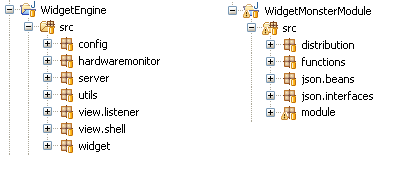
\includegraphics[width=10cm]{screenshot_2_projects}
  \caption{Project Structure}
  \label{fig:projects}
\end{figure}

\noindent
The following listing briefly describes the single packages of both projects in alphabetical order to give an overview of the implementation:
\\
\\
\textbf{config} 
\\
Lorem Ipsum...
\\
\\
\textbf{server} 
\\
Lorem Ipsum...
\\
\\
\textbf{utils} 
\\
Lorem Ipsum...

\section{Important Implementation Aspects\label{sec:implaspects}}

Do not explain every class in detail. Give a short introduction about the modules or the eclipse projects. If you want to explain relevant code snippets use the 'lstlisting' tag of LaTeX. Put only short snippets into your thesis. Long listing should be part of the annex.

\lstset{caption=JSON String Code Snippet,label=jsonstring,showstringspaces=false}
\begin{lstlisting}
{
	id: 1,
	method: "myInstance.getGroup",
	params: ["Teammates", 2, true]
}

{
	id: 2,
	result: [
		  "groupDesc":"These are my teammates",
		  {
			"javaClass":"src.package.MemberClass",
			"memberName": "Bob",      
		  }
		]
}\end{lstlisting}

You can also compare different approaches. Example: Since the implementation based on X failed I choosed to implement the same aspect based on Y. The new approach resulted in a much faster ...

\section{Graphical User Interface\label{sec:gui}}

Lorem Ipsum...

\section{Documentation\label{sec:docu}}

Lorem Ipsum...


